\documentclass[12pt, a4paper]{report}
\usepackage[polish]{babel}
\usepackage[utf8]{inputenc}
\usepackage{graphicx,wrapfig, lipsum}
\usepackage{a4wide}
\usepackage{titlesec}
\usepackage[T1]{fontenc}
\usepackage{adjustbox}
\usepackage{multirow}
\usepackage[table,xcdraw]{xcolor}
\usepackage{hyperref}
\usepackage{enumitem}
\usepackage{float}
\usepackage{geometry}
\usepackage{xcolor}
\usepackage[cache=false]{minted}
\usepackage{listings}
\usepackage{amsmath} 
\usepackage{amssymb}
\usepackage{xurl}
\usepackage{chngcntr}
\usepackage{tabularx}
\usepackage{fancyhdr}

\setminted[python]{
    frame=single,
    framesep=1mm,
    rulecolor=\color{lightgray}
}

% SET UP ARIAL FONT -----------------------------------------------------------------
\renewcommand{\rmdefault}{phv} 
\renewcommand{\sfdefault}{phv} 

% HEADER AND FOOTER SETTINGS ---------------------------------------------------------
\pagestyle{fancy}
\fancyhead{} 
\fancyfoot{} 
\fancyfoot[L]{\textcolor{darkgray}{Security of Computer Systems - 2026}}

\renewcommand{\headrule}{\hbox to \headwidth{\color{darkgray}\rule{16cm}{0.4pt}\hfill}}
\renewcommand{\footrule}{\hbox to \headwidth{\color{darkgray}\rule{16cm}{0.4pt}\hfill}}
% -------------------------------------------------------------------------------------

\counterwithin{figure}{section}
\makeatletter
\renewcommand{\thefigure}{\thesection\arabic{figure}}
\usemintedstyle{autumn}


\geometry{
    left = 25mm,
    right = 25mm,
    top = 25mm,
    bottom = 25mm,
    headsep=15mm % DOES THIS WORK?????
}
\setcounter{secnumdepth}{3}
\renewcommand{\thesection}{\arabic{section}.}
\renewcommand{\thesubsection}{\arabic{section}.\arabic{subsection}.}
\renewcommand{\thesubsubsection}{\arabic{section}.\arabic{subsection}.\arabic{subsubsection}.}

\titleformat*{\section}{\LARGE\bfseries}
\renewcommand{\figurename}{Rys}
\setlength{\intextsep}{2cm}
\setlength{\textfloatsep}{0cm}

\begin{document}

% -------------------------------------------------------------------------------
\newpage
\begin{center}

\textcolor{white}{x} % is there a better way for it? definetely? do i feel like looking for it when this works? absolutely not
\vspace{65mm}

{\fontsize{24pt}{28pt}\selectfont {\textbf{Security of Computer Systems}} }
\\
\vspace{37,5mm}
{\fontsize{18pt}{21pt}\selectfont {\textbf{Project Report}} }
\vspace{76mm}
\\
{\fontsize{12pt}{15pt}\selectfont
Authors:\\
Alicja Sobiech, 188861\\
Miłosz Gonsior, 193475
\\
\vspace{10mm}
Version: 2.5
}

\end{center}
\newpage
% -------------------------------------------------------------------------------

% ----------------------------------- DOCUMENT VERSIONS ----------------------------------

{\fontsize{13pt}{16pt}\selectfont
\subsection*{Versions}}

{\fontsize{11pt}{13pt}\selectfont

\setlength{\tabcolsep}{11pt}
\renewcommand{\arraystretch}{1.4}
\newcolumntype{Y}{>{\centering\arraybackslash}X}

\begin{adjustbox}{center, nofloat=figure,vspace=\bigskipamount}
\begin{tabularx}{\textwidth}{|c|c|Y|}
\hline
\textbf{Versions} & \textbf{Date} & \textbf{Description of changes} \\ \hline
1.0               & 04.04.2026      & Creation of document \\ \hline
1.1               & 07.04.2026      & Filling out the control meeting section \\ \hline
2.0               & 17.05.2026      & Translating the document from .docx to .tex \\ \hline
2.1               & 31.05.2026      & Initial version of section 2  \\ \hline
2.2               & 07.06.2026      & Filling out section 2 \\ \hline
2.3               & 08.06.2026      & Completing the bibliography \\ \hline
2.4               & 08.06.2026      & Completing section 2 \\ \hline
2.5               & 08.06.2026      & Final formatting improvements \\ \hline
\end{tabularx}
\end{adjustbox}
}


% ---------------------------------------------------------------------------------
% PAPER ITSELF --------------------------------------------------------------------
% ---------------------------------------------------------------------------------
\newpage
\titleformat{\section} {\fontsize{16pt}{19pt}\selectfont\bfseries} {\thesection}{1em}{}
\titleformat{\subsection} {\fontsize{13pt}{16pt}\selectfont\bfseries} {\thesubsection}{1em}{}

\titleformat{\subsubsection} {\fontsize{12pt}{15pt}\selectfont\bfseries} {\thesubsubsection}{1em}{}

\section{Project - control term}
\subsection{Description}
The aim of the overall project is the implementation of a set of applications emulating an environment with trusted third party (TTP), server and a client.

\subsection{Results - implemented functionalities}
\begin{itemize}
    \item Docker configuration
    \item Basic version of server and TTP applications
    \item RSA key pair generation
\end{itemize}

\subsection{Plans for future work}
\begin{itemize}
    \item Design and implementation of a Graphical User Interface (GUI)
    \begin{itemize} % TODO - CHANGE THSI STYLE TO CIRCLE (AND CHANGE REGULAR TO BIGGER ONE)
        \item Icons presenting the state of the application
    \end{itemize}
    \item Implementation of the Client
    \item Running tests (eg. sample attacks)
    \item Generation of documentation using Doxygen

\end{itemize}

\newpage
\section{Project - Final term}
\subsection{Achieved results}
The result of our work is the developement of 3 python applications emulating a user/client, a server and a trusted third part (TTP) according to the project instruction \(^{\text{[1]}}\). The network enviroment is created using Docker containers. The cryptographic tasks are done using the \mintinline{text}{cryptography} package.
\\\\ \noindent
The main application is the client service and it's GUI. It allows for authentication cia the trusted third party (TTP), obtaining an AES key and sending encypted messages to the server application.
\\\\ \noindent
The TTP and Server application work in the background in relation to the Client service.
The main tasks of the TTP service is generating certificates and facilitating authorisation attempts. The Server service receives and decrypts messages from the user.

\subsection{Key functionalities}

\subsubsection{Key handling}
4096-bit keys are generated as a private, public pair using \mintinline{python}{generate_private_key()} and  \mintinline{python}{public_key()} methods respectively.
\\AES key is generated using \mintinline{python}{urandom()} method.

\begin{minted}{python}
def generate_RSA_key_pair():
    private_key = rsa.generate_private_key(
        public_exponent=65537,
        key_size=4096)
    public_key = private_key.public_key()
    return public_key, private_key

def generate_aes_key():
    return os.urandom(32)
\end{minted}
\begin{center}
List.1 RSA and AES key generation
\end{center}

\vspace{4pt}

\noindent
The key serialization converts them into PEM-encoded bytes. The public key is encrypted during this process while the private key remains without encryption. 
Deserialization is done using \mintinline{python}{load_pem_public_key()} and \mintinline{python}{load_pem_private_key()} methods.

\begin{minted}{python}
def serialize_public_key(public_key):
return public_key.public_bytes(
    encoding=serialization.Encoding.PEM,
    format=serialization.PublicFormat.SubjectPublicKeyInfo)

def deserialize_public_key(serialized_public_key):
    return serialization.load_pem_public_key(serialized_public_key)
\end{minted}
\begin{center}
List.2 Public key serialization and deserialization
\end{center}

\newpage

\begin{minted}{python}
def serialize_private_key(private_key):
    return private_key.private_bytes(
        encoding=serialization.Encoding.PEM,
        format=serialization.PrivateFormat.PKCS8,
        encryption_algorithm=serialization.NoEncryption())

def deserialize_private_key(serialized_private_key):
    return serialization.load_pem_private_key(
        serialized_private_key, 
        password=None)
\end{minted}
\begin{center}
List.3 Private key serialization and deserialization
\end{center}

\subsubsection{Certificate handling}

The certificate is generated using \mintinline{python}{x509.CertificateBuilder()} using the given public key of the certificate subject and signed using the issuer's private key. Certificate generated in that way is valid for 4 weeks from the moment of generation.
\begin{minted}{python}
def generate_certificate(subject_id, subject_public_key,
                        issuer_id, issuer_private_key):
    builder = x509.CertificateBuilder()
    
    builder = builder.subject_name(x509.Name(
                [x509.NameAttribute(NameOID.COMMON_NAME, subject_id)]))
    builder = builder.issuer_name(x509.Name(
                [x509.NameAttribute(NameOID.COMMON_NAME, issuer_id)]))
    builder = builder.public_key(subject_public_key)
    builder = builder.serial_number(x509.random_serial_number())
    builder = builder.not_valid_before(datetime.datetime.now())
    builder = builder.not_valid_after(
                datetime.datetime.now() + datetime.timedelta(weeks=4))

    return builder.sign(issuer_private_key, hashes.SHA256())
\end{minted}
\begin{center}
List.4 Certificate generation
\end{center}

\noindent
A certificate generated in the way described above can also be serialized and later deserialized. These processes are done with \mintinline{python}{cert.public_bytes()} and\\  \mintinline{python}{x509.load_pem_x509_certificate()} methods respectively.

\begin{minted}{python}
def serialize_certificate(cert):
    return cert.public_bytes(serialization.Encoding.PEM)

def deserialize_certificate(serialized_cert):
    return x509.load_pem_x509_certificate(serialized_cert)
\end{minted}
\begin{center}
List.5 Certificate serialization and deserialization
\end{center}

\subsubsection{Data encryption and decryption}

Data can be encrypted and decrypted in two ways: using RSA (Rivest-Shamir-Adleman algorithm) with OAEP padding and SHA-256 algorithm or using AES (Advanced Encryption Standard) with CFB mode (Cipher Feedback Mode).

\begin{minted}{python}
def encrypt_data(public_key, data):
    return public_key.encrypt(
        data,
        padding.OAEP(
            mgf=padding.MGF1(algorithm=hashes.SHA256()),
            algorithm=hashes.SHA256(),
            label=None 
        ) 
    )

def decrypt_data(private_key, encrypted_data):
    return private_key.decrypt(
        encrypted_data,
        padding.OAEP(
            mgf=padding.MGF1(algorithm=hashes.SHA256()),
            algorithm=hashes.SHA256(),
            label=None
        ) 
    )
\end{minted}
\begin{center}
List.6 Data encryption and decryption using RSA-OAEP with SHA-256 
\end{center}

\begin{minted}{python}
def encrypt_aes(key, plaintext):
    iv = os.urandom(16)
    cipher = Cipher(algorithms.AES(key), modes.CFB(iv))
    encryptor = cipher.encryptor()
    ciphertext = iv + encryptor.update(plaintext) + encryptor.finalize()
    return ciphertext

def decrypt_aes(key, ciphertext):
    iv = ciphertext[:16]
    cipher = Cipher(algorithms.AES(key), modes.CFB(iv))
    decryptor = cipher.decryptor()
    plaintext = decryptor.update(ciphertext[16:]) + decryptor.finalize()
    return plaintext
\end{minted}
\begin{center}
List.7 Data encryption and decryption using AES
\end{center}

\newpage
\subsection{Regular flow test}
Regular flow test of our system is conducted by realizing the following steps:\\

\noindent
\begin{minipage}[]{0.5\textwidth}
\begin{enumerate}
    \item Click the "\mintinline{text}{Log in with TTP}"\(\ \) button
    \item Click the "\mintinline{text}{Download AES key}"\(\ \) button
    \item Type a message into the textbox
    \item Click the "\mintinline{text}{Send message}"\(\ \) button
\end{enumerate}

\vspace{50pt}

\end{minipage}\hfill
\hspace{0.05\textwidth}
\begin{minipage}[c]{0.45\textwidth}
\begin{center}
    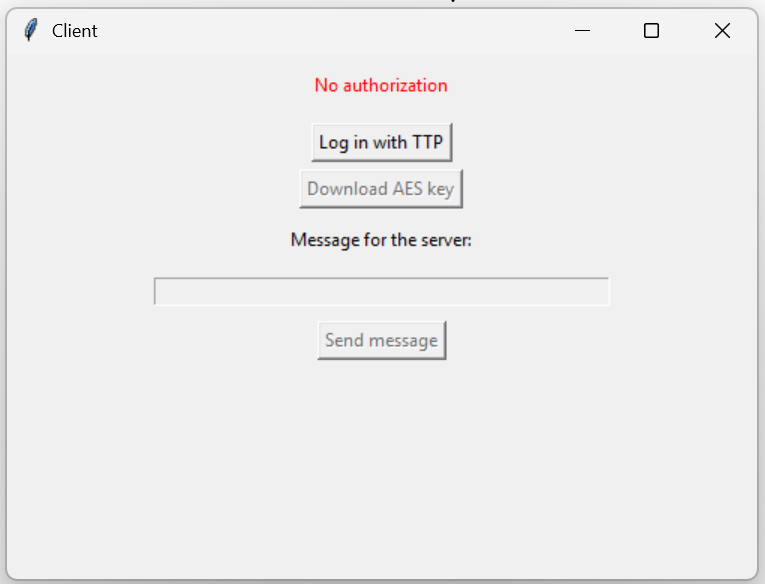
\includegraphics[width = \textwidth]{flow_test/0.png}

Fig.1 Client app before flow test
\end{center}
\end{minipage}

\vspace{10pt}
\noindent
\begin{minipage}[]{0.475\textwidth}
\begin{center}
    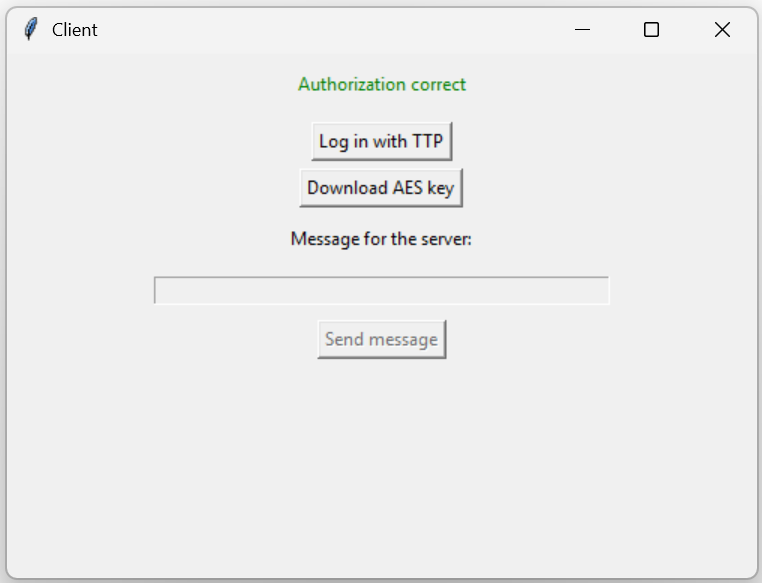
\includegraphics[width = \textwidth]{flow_test/1.png}

Fig.2 GUI state after step 1
\end{center}
\end{minipage}\hfill
\hspace{0.05\textwidth}
\begin{minipage}[c]{0.475\textwidth}
\begin{center}
    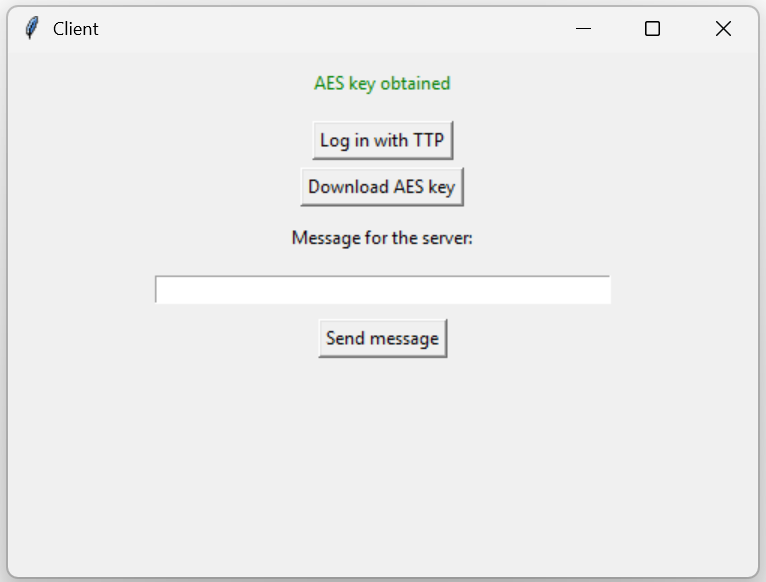
\includegraphics[width = \textwidth]{flow_test/2.png}

Fig.3 GUI state after step 2
\end{center}
\end{minipage}

\vspace{10pt}

\noindent
\begin{minipage}[]{0.475\textwidth}
\begin{center}
    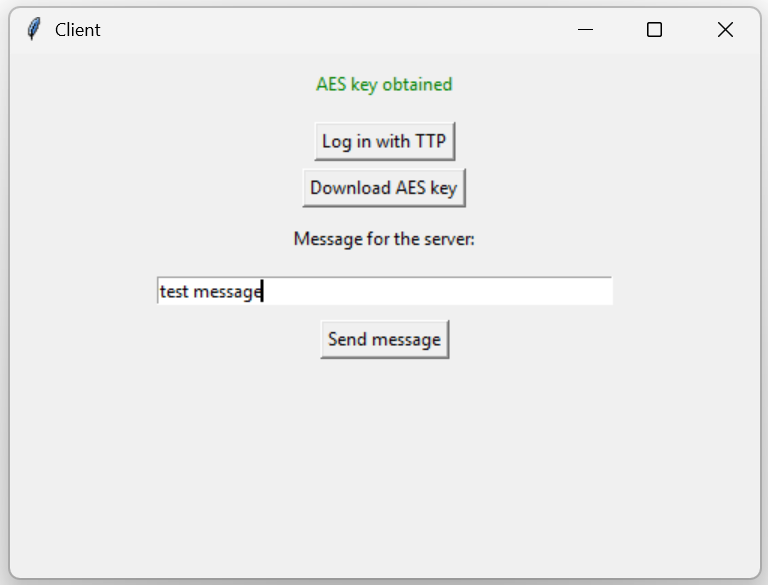
\includegraphics[width = \textwidth]{flow_test/3.png}

Fig.4 GUI state after step 3
\end{center}
\end{minipage}\hfill
\hspace{0.05\textwidth}
\begin{minipage}[c]{0.475\textwidth}
\begin{center}
    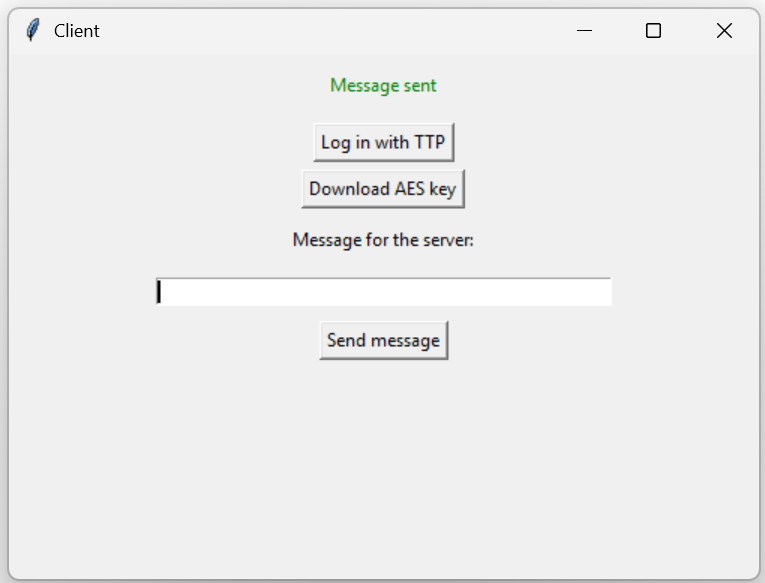
\includegraphics[width = \textwidth]{flow_test/4.png}

Fig.5 GUI state after step 4
\end{center}
\end{minipage}

\begin{center}
    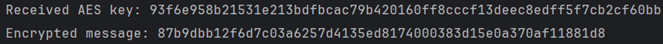
\includegraphics[width = \textwidth]{flow_test/5_guiCons.png}

Fig.6 Client app console after step 4
\end{center}

\begin{center}
    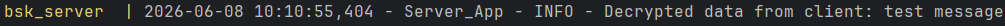
\includegraphics[width = \textwidth]{flow_test/6_serverMess.png}

Fig.7 Decrypted message in server console after step 4
\end{center}

\subsection{Performed vulnerability tests and their results}

\subsubsection{Mismatch of client IDs between TTP and the server}


\noindent
\begin{minipage}[]{0.475\textwidth}
In order to test how our applications behave when client IDs sent to the server and TTP are different we temporarily modified our code, so that TTP recieved the correct client ID, and the server recieved a fake ID.\\\\ \noindent As a result we were not able to obtain the AES key. 

\vspace{60pt}

\end{minipage}\hfill
\hspace{0.05\textwidth}
\begin{minipage}[c]{0.475\textwidth}
\begin{center}
    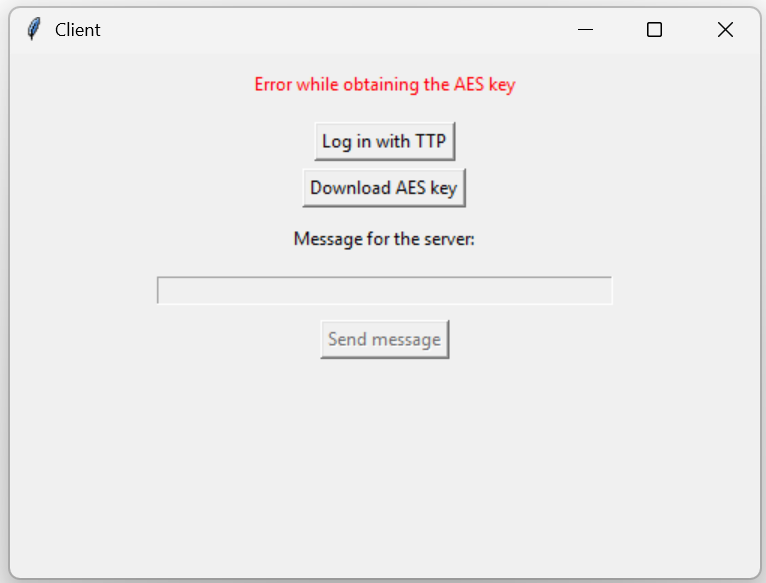
\includegraphics[width = \textwidth]{tests/incorrect_client/1stateAfterAES.png}

Fig.8 GUI state after attempting to obtain an AES key
\end{center}
\end{minipage}

\begin{minted}{python}
client_id = crypto.generate_random_id()
    
s.connect((server_host, server_port))
payload = { "type": "service_request", "client_id": "fake ID" }

ttp_s.connect((ttp_host, ttp_port))
payload={ "type": "fetch_key", "client_id": client_id }
\end{minted}
\begin{center}
List.8 Payloads for server (\mintinline{python}{s}) and ttp (\mintinline{python}{ttp_s}) simulating mismatch in client IDs
\end{center}

\subsubsection{Forged certificate}

??? do we even have certificate checking

\subsection{Summary}

% ---------------------------------------------------------------------------------
% ZRODLA --------------------------------------------------------------------------
% ---------------------------------------------------------------------------------
\newpage
\section*{Literature}
\renewcommand{\labelenumi}{[\arabic{enumi}]}
\begin{enumerate}

\item Rajchowski P.: \textit{Security of Computer Systems - Project. Emulating environment with Trusted Thrid Party and Client-Server data exchange scenario} [Project instruction], Gdańsk (Gdańsk University of Technology), 23.02.2026

\item Online \textit{Doxygen} documentation, [accessed on 07.06.2026], Aviable at: \url{https://www.doxygen.nl/manual/lists.html}

\item Online \textit{cryptography} documentation, [accessed on 07.06.2026], Aviable at: \url{https://cryptography.io/en/latest/}

\item Mumba E.: \textit{Mastering Python Function Documentation: A Practical Guide}, In: DeepDocs, 15.11.2025 [accessed on 07.06.2026], Aviable at: \url{https://deepdocs.dev/function-documentation-python/}

\item \textit{Privacy-Enhanced Mail}, In: Wikipedia, [online], 27.02.2026, [accessed on 06.06.2026], Aviable at: \url{https://en.wikipedia.org/wiki/Privacy-Enhanced_Mail}

\item \textit{X.509}, In: Wikipedia, [online], 22.04.2026, [accessed on 07.06.2026], Aviable at: \url{https://en.wikipedia.org/wiki/X.509}

\item \textit{SHA-2}, In: Wikipedia, [online], 24.05.2026, [accessed on 07.06.2026], Aviable at: \url{https://en.wikipedia.org/wiki/SHA-2}

\item Moriarty K. et al.:\textit{PKCS \#1: RSA Cryptography Specifications Version 2.2}, In: RFC Editor, United States, 01.11.2016, 8017, ISSN: 2070-1721, Aviable at: \url{https://doi.org/10.17487/RFC8017}

\item \textit{RSA Algorithm in Cryptography}, In: GeeksForGeeks, 23.07.2025, [accessed on 07.06.2026], Aviable at: \url{https://www.geeksforgeeks.org/computer-networks/rsa-algorithm-cryptography/}

\item Abhinand S.: \textit{Advanced Encryption Standard (AES)}, In: GeeksForGeeks, 08.08.2025, [accessed on 07.06.2026], Aviable at: \url{https://www.geeksforgeeks.org/computer-networks/advanced-encryption-standard-aes/}

\item Kattamuri M.: \textit{Block Cipher modes of Operation}, In: GeeksForGeeks, 30.05.2026, [accessed on 07.06.2026], Aviable at: \url{https://www.geeksforgeeks.org/ethical-hacking/block-cipher-modes-of-operation/}

\end{enumerate}

\end{document}
